% Copy this section into the manuscript, or use \input{...}.
% Required in the manuscript preamble:
% \usepackage{amsmath,amssymb,graphicx,booktabs,tikz,placeins}
% \usetikzlibrary{arrows.meta}
% Put the accompanying figures directory beside the main manuscript.

\section{Numerical Experiments}
\label{sec:numerical-experiments}

We evaluate the proposed joint-coincidence estimator (\jce) and marginal-coincidence estimator (\mce) through quantum circuit simulations using Qiskit~\cite{javadiabhari2024quantumcomputingqiskit}. We first consider a three-link star network and compare the estimation accuracy of the proposed methods with two existing tomography methods: \mergecast~\xw{cite}, which supports general Pauli-channel tomography, and Multicast~\cite{deandrade2024quantumnetworktomography}, which is restricted to depolarizing-channel tomography. The comparisons are conducted under different measurement budgets and assumptions about prior channel knowledge. We also examine the number of fidelity-improved entangled pairs retained during distillation to demonstrate the dual functionality of the proposed methods. We then extend \jce to a six-link triangular network \xw{(Figure~\ref{})} to evaluate its applicability beyond the three-link star topology. Estimation accuracy is quantified by the mean squared error (MSE) of the estimated Pauli-channel parameters, with measurement outcomes generated during distillation reused for channel estimation.
\subsection{Performance in a Three-Link Star Network}
\label{subsec:star-experiments}

\subsubsection{Network setting}
We consider a three-link star network in which each link is modeled by a depolarizing channel with \(q_{X,\ell}=q_{Y,\ell}=q_{Z,\ell}\). The channel parameters are \(q_{P,1}=0.88\), \(q_{P,2}=0.86\), and \(q_{P,3}=0.84\) for links 1, 2, and 3, respectively. 

Local gates and measurements are assumed to be ideal.
We consider two estimation settings that differ in whether the
depolarizing structure is known beforehand. Each measurement
budget is evaluated using 1000 Qiskit trials.

The measurement budget counts all measured qubits, including
those measured in rejected distillation attempts, and excludes
retained output pairs and unmeasured qubits discarded at
the central node.
For JCE and MCE, these measurements are part of distillation;
for the baseline protocols, they are dedicated to tomography.
Thus, ``free distillation measurement'' denotes reuse without
additional tomography measurements, rather than zero
physical resource consumption.

\paragraph{Without a depolarizing prior.}
Although the simulated channels are depolarizing, the estimators  in Fig.~\ref{fig:star-tomography-comparisons}(a)
are only supplied with the general Pauli-channel model.
JCE, MCE, and Mergecast therefore independently
estimate all nine parameters
$\{q_{P,\ell}:P\in\{X,Y,Z\},\,\ell=1,2,3\}$,
without imposing equality between the three Pauli components.

A complete round uses four, nine, and nine configurations for
JCE, MCE, and Mergecast, respectively, and 
16, 36, and 9 measurements.
Their performance is compared at equal measurement budgets.



The MSE decreases as the measurement budget increases.
Mergecast achieves the lowest MSE in this setting, while
JCE is more accurate than MCE at the same measurement budget.
The proposed estimators additionally use their measurement
records for distillation, producing the retained entangled
pairs discussed below.
% Required packages: \usepackage{booktabs,threeparttable}
% Table fragment; requires \usepackage{booktabs}.
\begin{table}
\centering
\caption{Mean numbers of fidelity-improved Bell pairs over 1,000 Qiskit trials at  approximately $200,000$ measurements per method. JCE and MCE use independent records, with four and nine configurations per round, respectively. Fidelities describe theoretical input and accepted-output ensembles. Mergecast retains no distilled outputs.}
\label{tab:three-methods-mean-retained-pairs}
\small
\setlength{\tabcolsep}{4pt}
\begin{tabular}{ccccc}
\toprule
$F_{\mathrm{in}}$ & $F_{\mathrm{out}}$ & JCE & MCE & Mergecast \\
\midrule
0.817600 & 0.901788 & 7,618 & 10,161 & 0 \\
0.804400 & 0.891105 & 7,355 & 9,800 & 0 \\
0.748456 & 0.843859 & 12,713 & 8,477 & 0 \\
\midrule
\multicolumn{2}{c}{Total} & \textbf{27,687} & \textbf{28,438} & \textbf{0} \\
\bottomrule
\end{tabular}
\end{table}

\begin{figure*}[tb]
\centering

\begin{subfigure}[t]{0.24\textwidth}
    \centering
    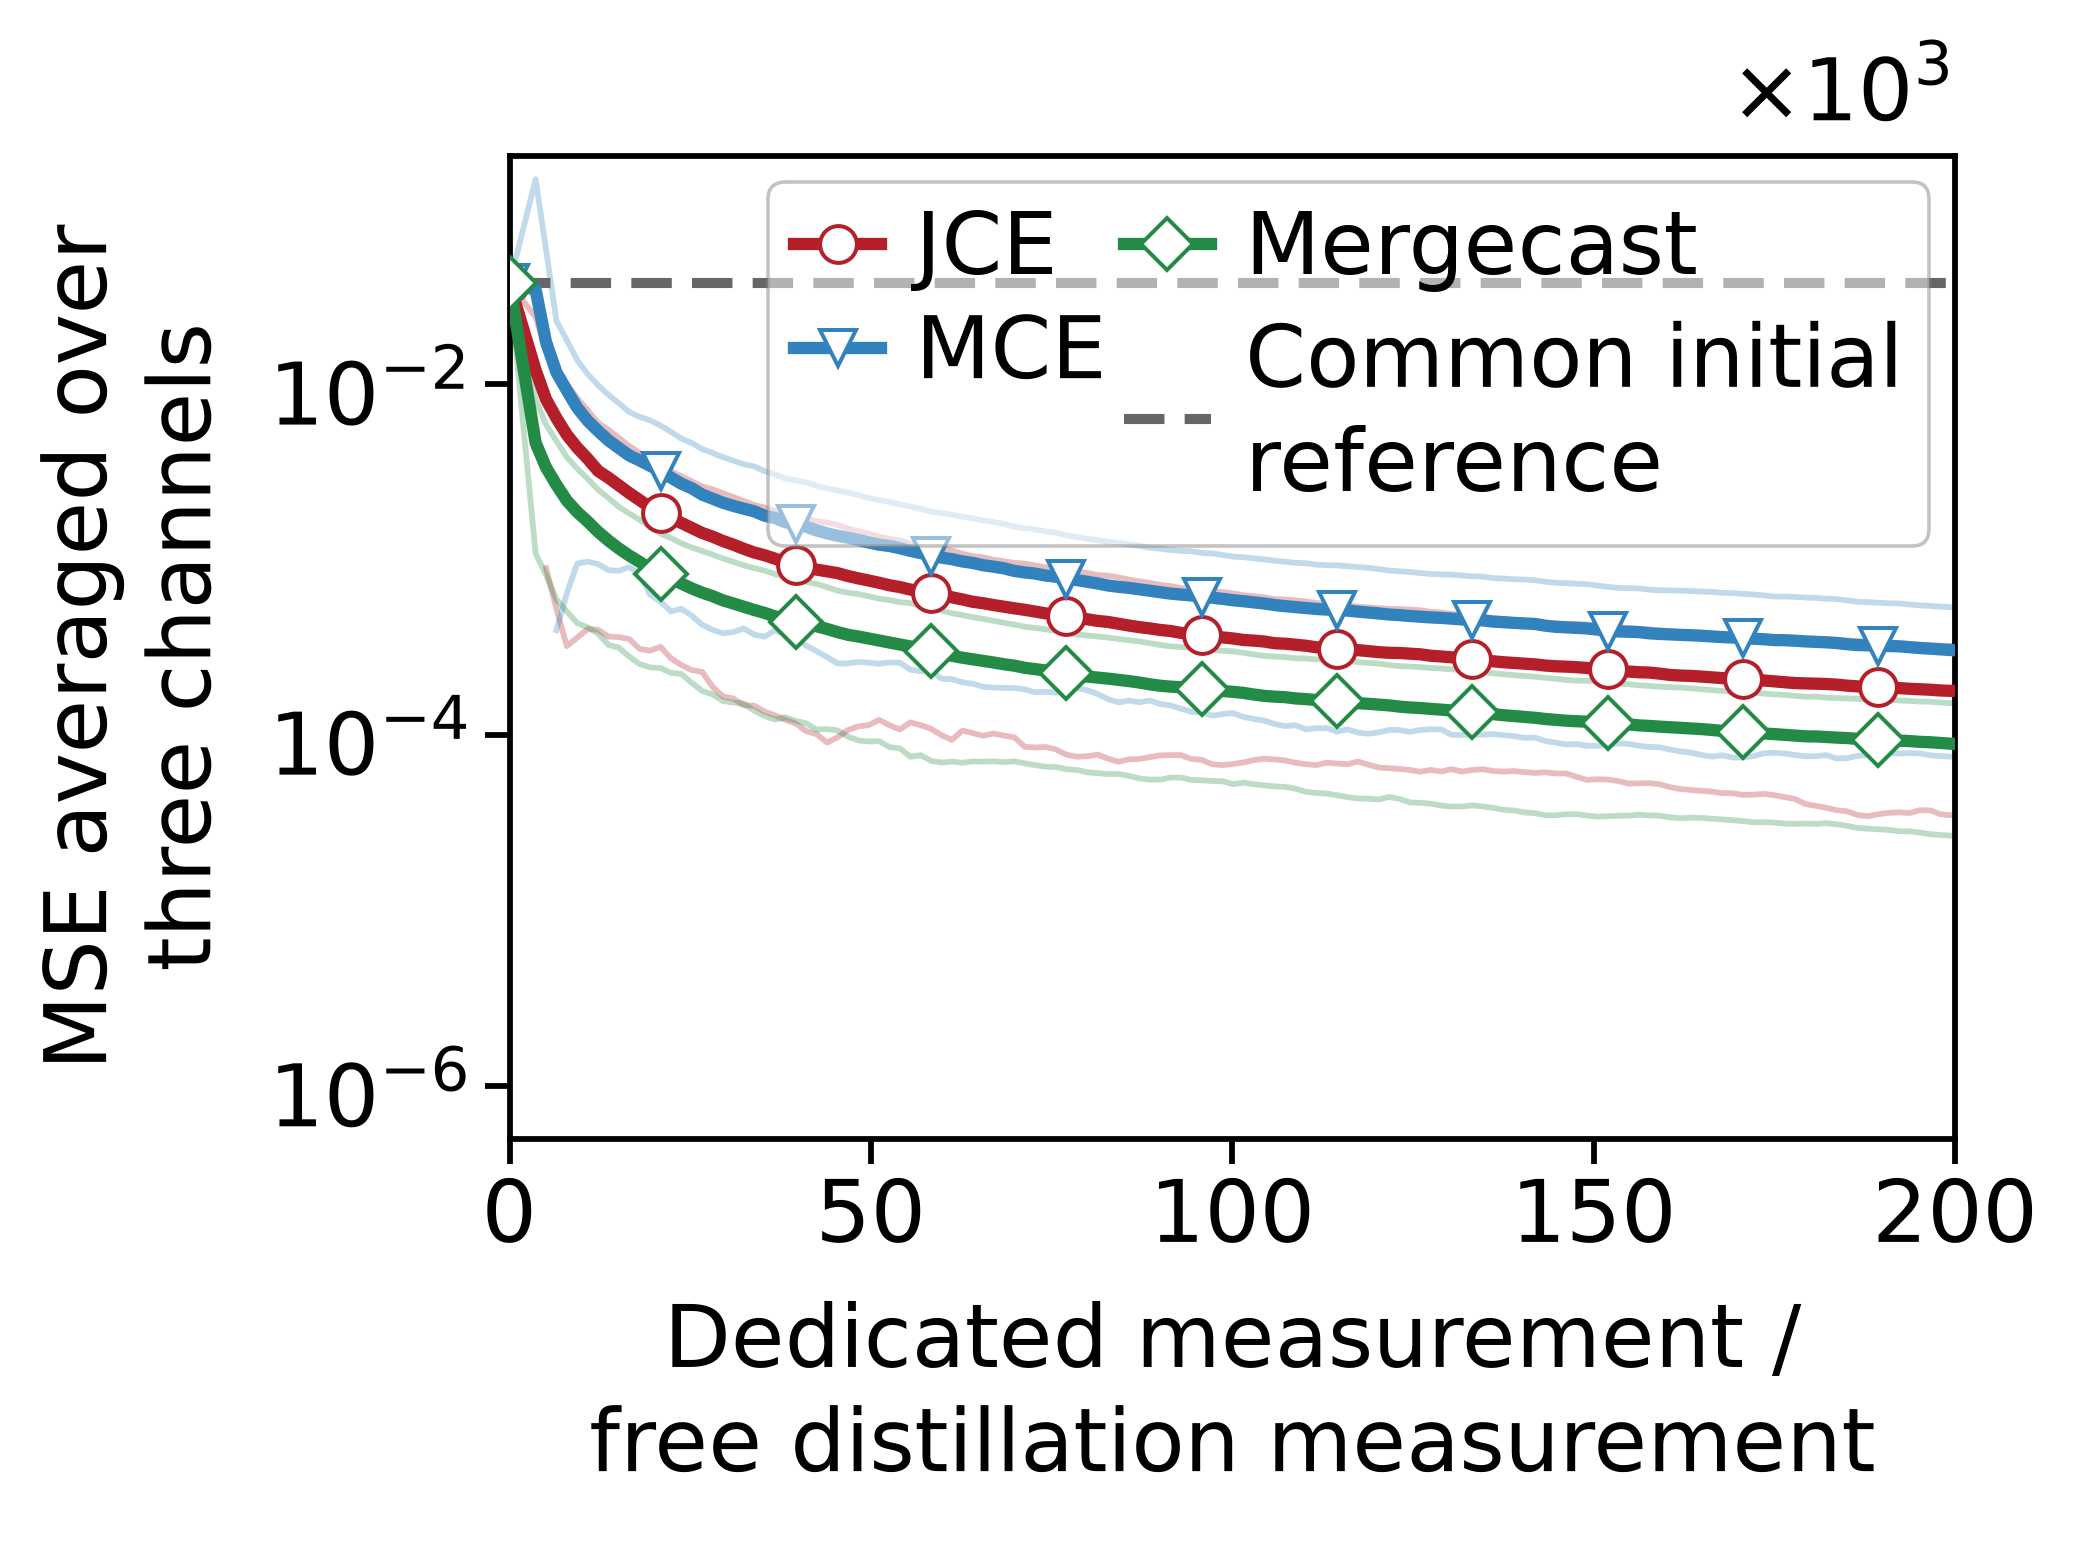
\includegraphics[width=\linewidth]
    {figures/star_three_methods_equal_measured_qubits.png}
    \caption{Without a depolarizing prior.}
    \label{fig:star-without-depolarizing-prior}
\end{subfigure}
\hfill
\begin{subfigure}[t]{0.24\textwidth}
    \centering
    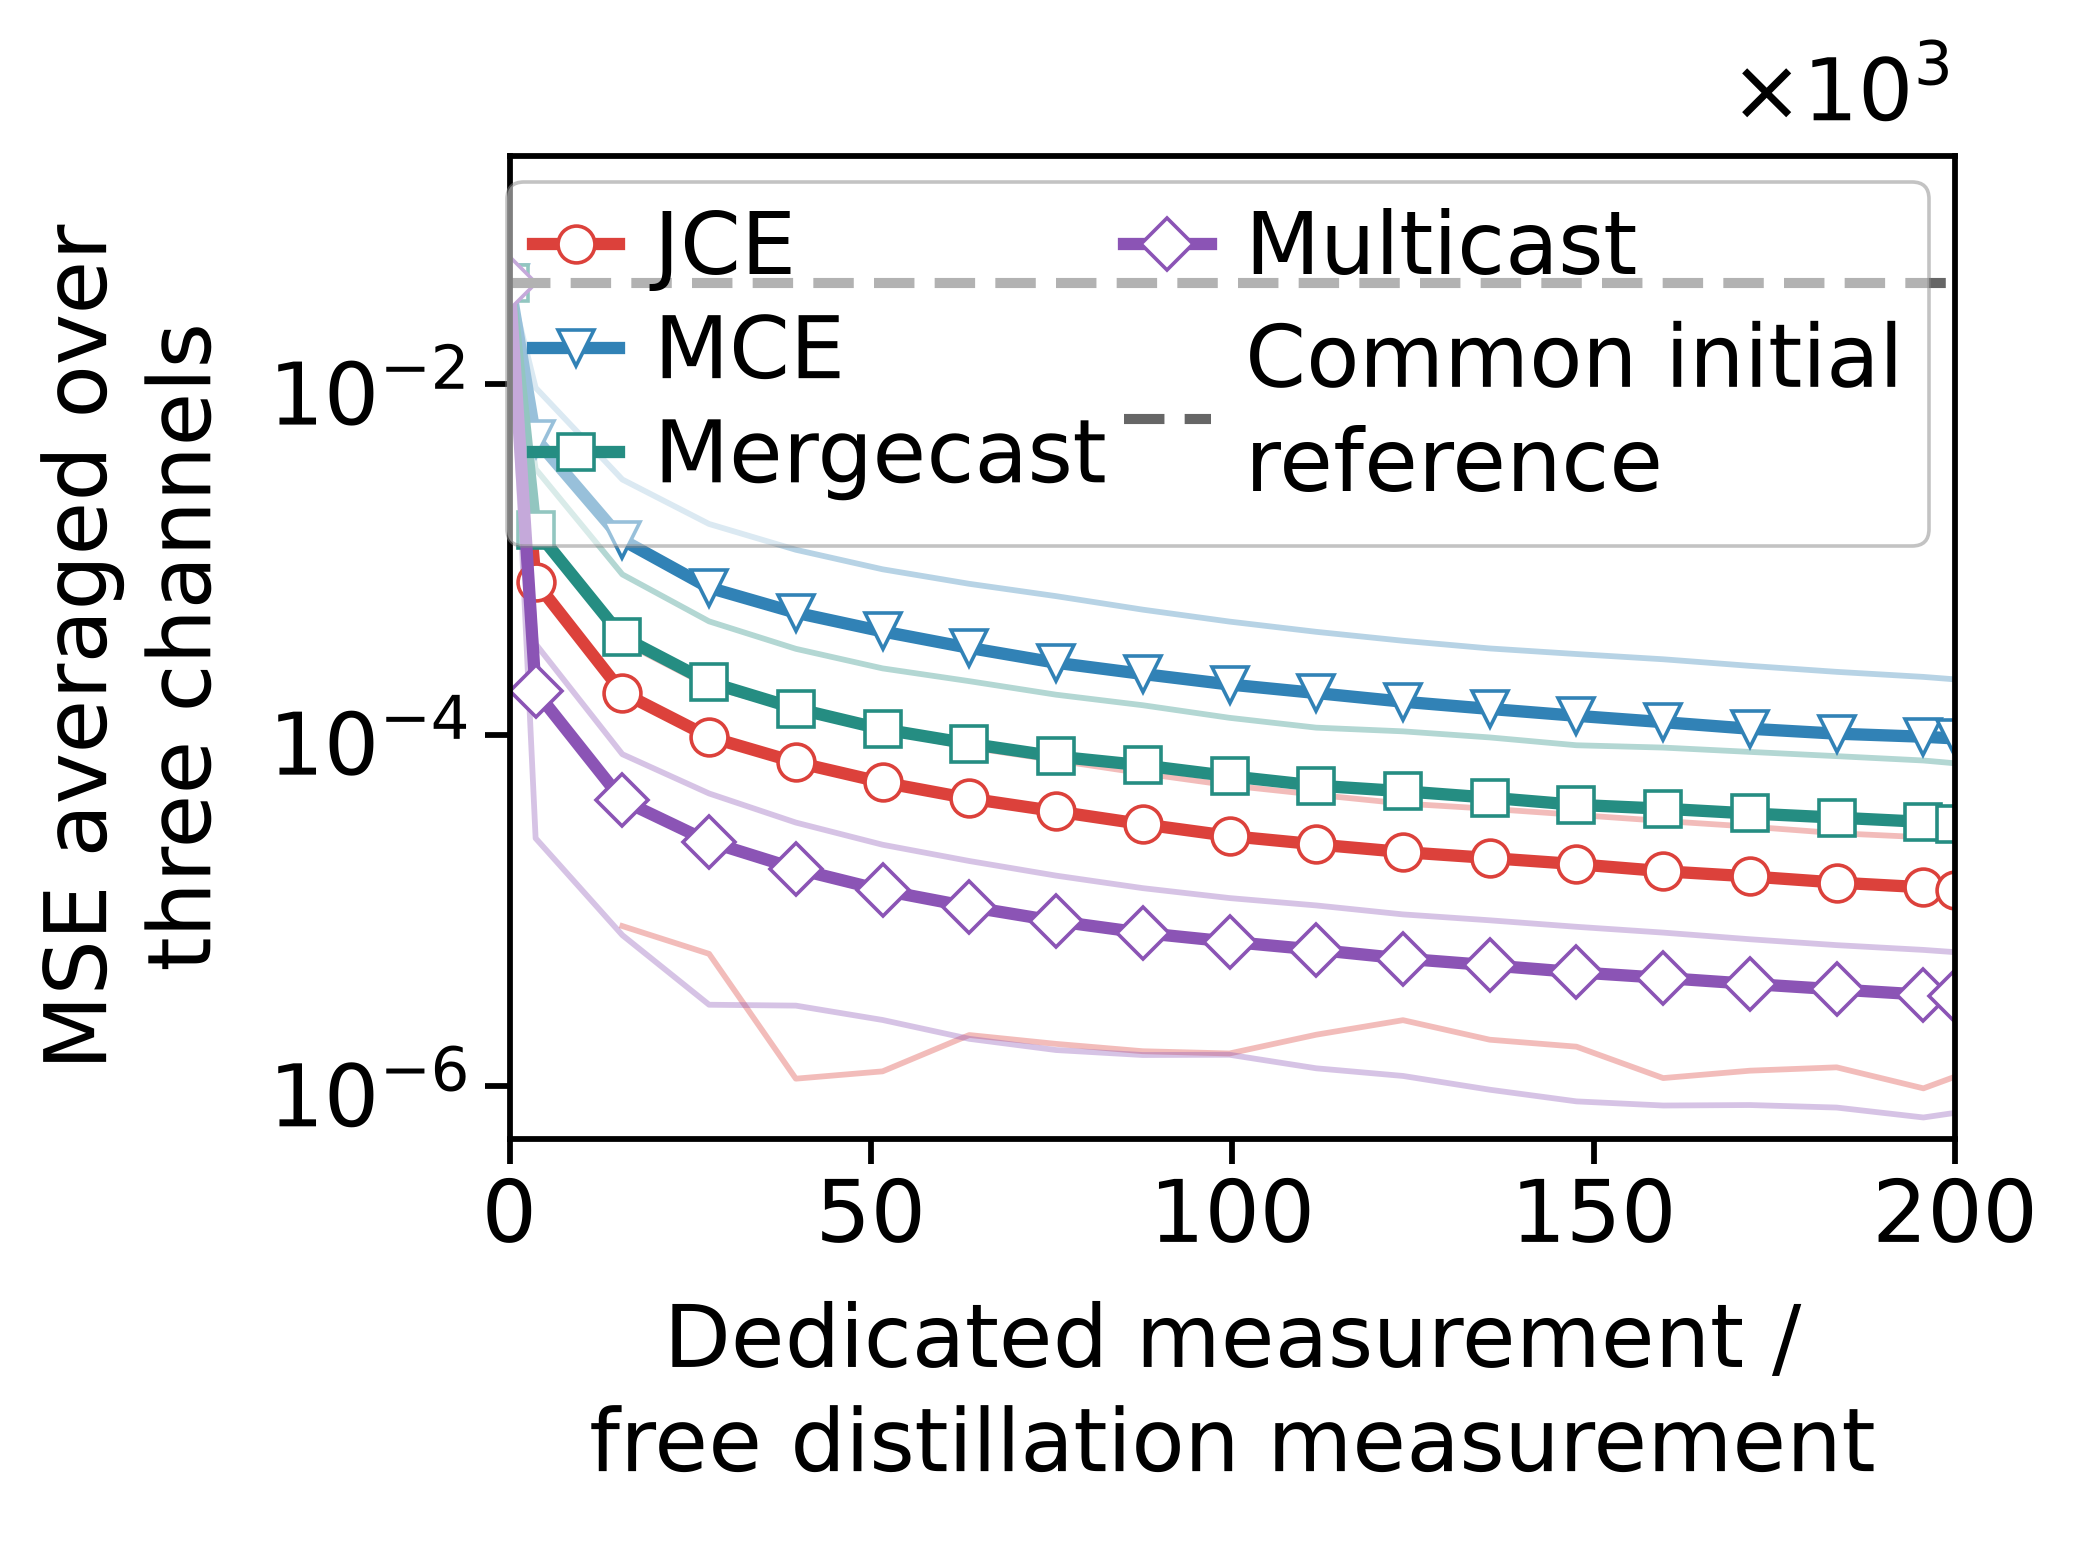
\includegraphics[width=\linewidth]
    {figures/comparison.png}
    \caption{With a depolarizing prior.}
    \label{fig:mergecast-measured-budget}
\end{subfigure}
\hfill
\begin{subfigure}[t]{0.24\textwidth}
    \centering
    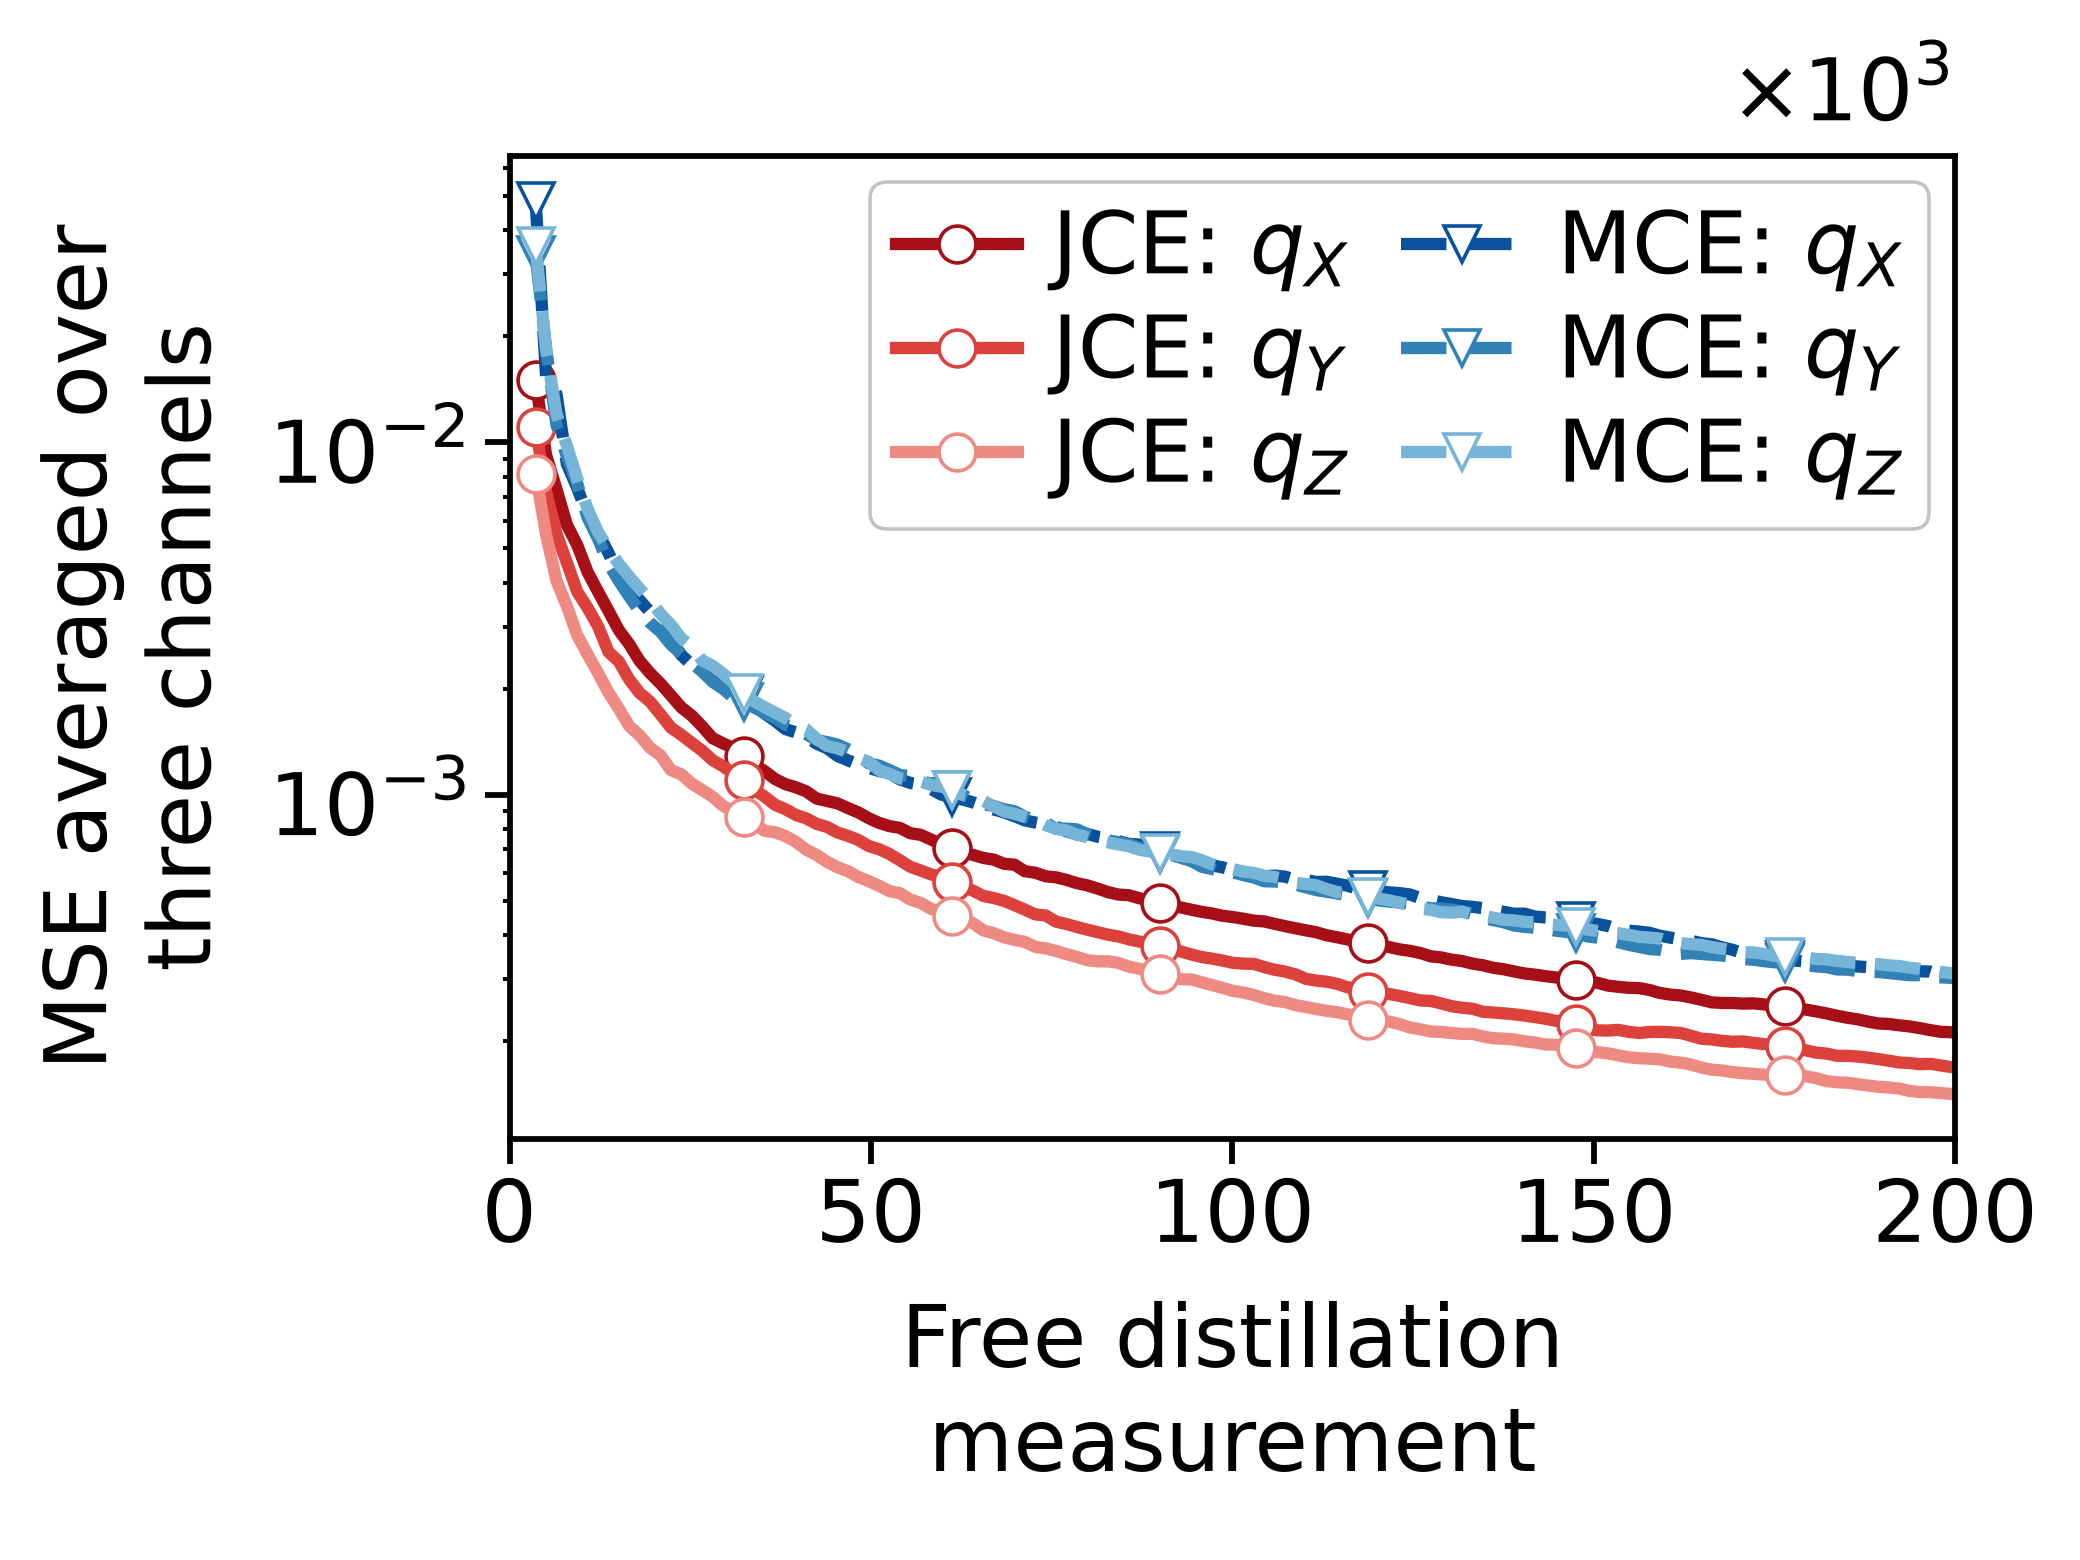
\includegraphics[width=\linewidth]
    {figures/estimator_component_mse_equal_measured_qubits.png}
    \caption{Equal round counts.}
    \label{fig:estimators-equal-rounds}
\end{subfigure}
\hfill
\begin{subfigure}[t]{0.24\textwidth}
    \centering
    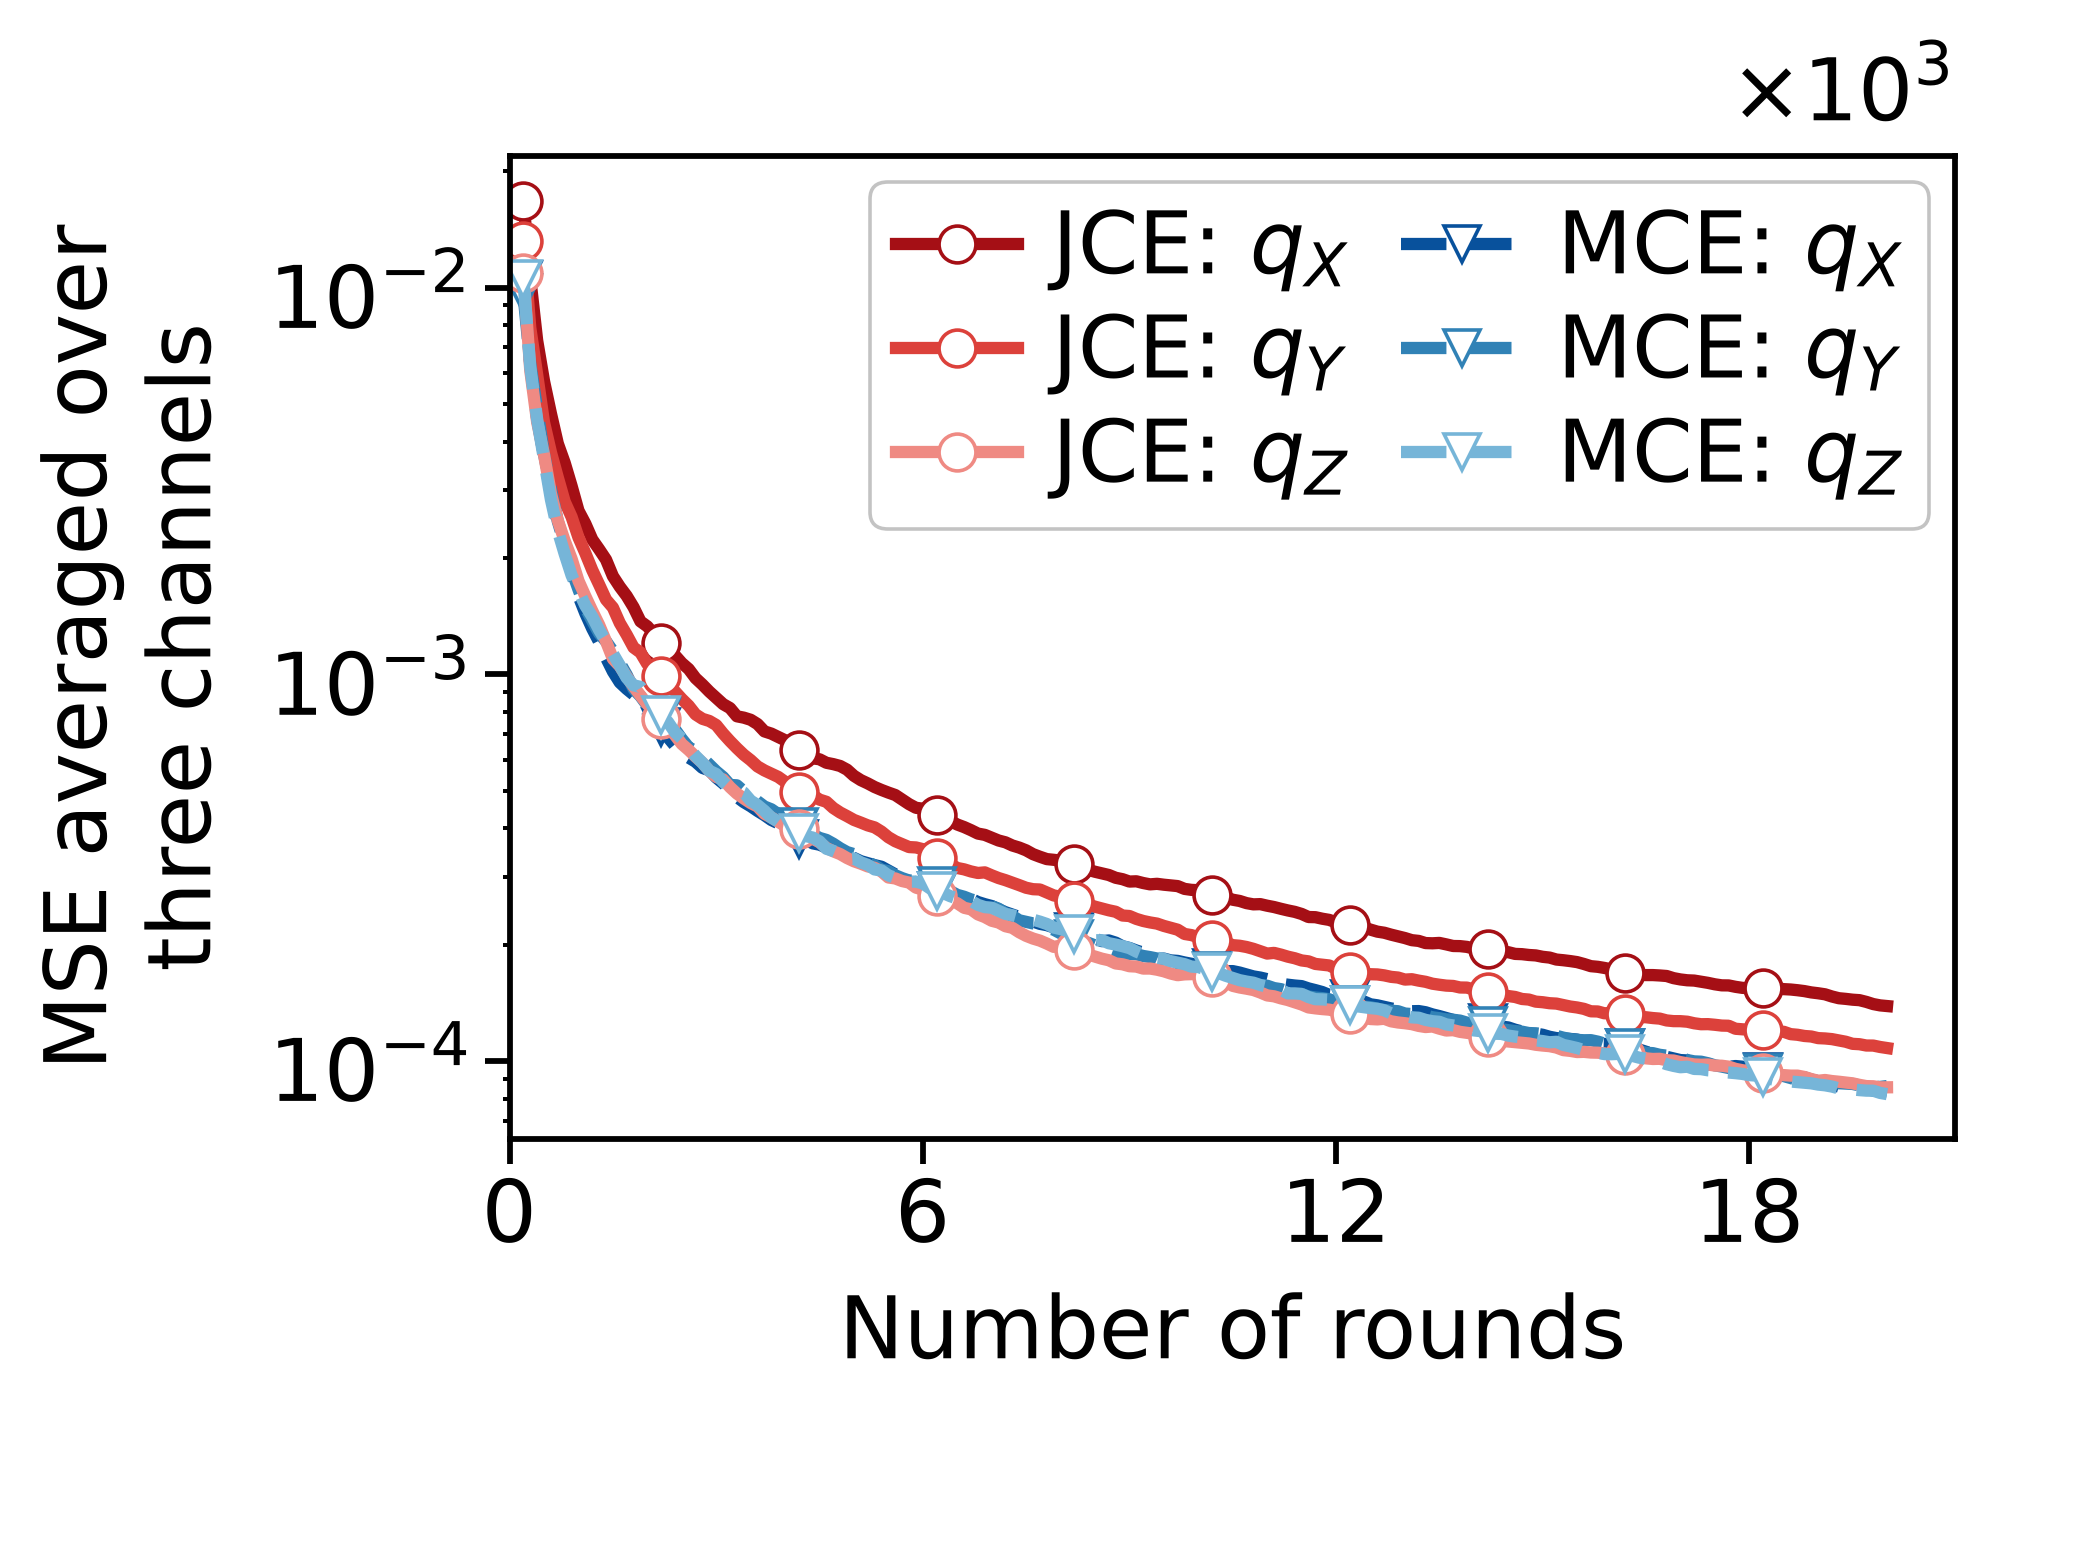
\includegraphics[width=\linewidth]
    {figures/estimator_component_mse_vs_rounds.png}
    \caption{Equal configuration counts.}
    \label{fig:estimators-equal-configurations}
\end{subfigure}

\caption{Tomography performance in the three-link star network.
(a) Comparison of JCE, MCE, and Mergecast
at equal measurement counts without a depolarizing prior,
using the MSE over nine independent Pauli parameters.
(b) Comparison with a known depolarizing model, where all methods
estimate three link parameters using maximum likelihood estimation.
Light curves in (a) and (b) indicate one standard deviation about
the mean; dashed horizontal lines mark the prescribed common
zero-data references.
(c) Component-wise MSE at equal round counts.
Each round executes four configurations for JCE
and nine for MCE.
(d) Component-wise MSE at equal numbers of configuration executions.
With $K$ executions, JCE performs $K/4$ rounds
and MCE performs $K/9$ rounds.
Component-wise errors are averaged over the three channels.
Each budget is evaluated using 1,000 Qiskit trials.}
\label{fig:star-tomography-comparisons}
\end{figure*}
\paragraph{With a depolarizing prior.}

Figure~\ref{fig:star-tomography-comparisons}(b) considers
the case in which all methods know the depolarizing structure.
Only the three parameters $(q_{P,1},q_{P,2},q_{P,3})$
are estimated, using maximum likelihood estimation.

The adapted JCE and MCE both execute three double-selection
configurations, $\rho_{12}$, $\rho_{13}$, and $\rho_{\mathrm m,23}$,
and measure 12 qubits per round.
JCE uses the joint $X/Z$ coincidence statistics, whereas
MCE uses the $Z$-coincidence marginal of the same records.
Mergecast uses two Unicast configurations and one Mergecast
configuration, measuring three qubits per round.
The Multicast baseline \cite{Andrade2024QNT} measures two
qubits per round.


Multicast achieves the lowest MSE, while JCE outperforms
Mergecast and MCE.
Because JCE and MCE use identical distillation records
in this setting, their difference demonstrates the benefit
of retaining the joint coincidence information for estimation.







% Table fragment for inclusion in the manuscript; not a standalone document.
% Requires \usepackage{booktabs} in the manuscript preamble.
% Generated from independent saved JCE/MCE records; no resampling or expected-count substitution.
% Row order: rho12, rho13, rho23_0

\subsubsection{Comparison of the two estimators}
Fig.~\ref{fig:star-tomography-comparisons}(c) and Fig.~\ref{fig:star-tomography-comparisons}(d) compare the
$X$-, $Y$-, and $Z$-component MSEs of JCE and MCE,
each averaged over the three links. Both estimators
reconstruct the channel parameters without imposing
the depolarizing constraint.

At equal measurement budgets, JCE achieves lower
component MSEs in this setting.
At equal round counts, MCE achieves lower MSEs for
the $X$ and $Y$ components, while the $Z$-component
MSEs are comparable.
For MCE, the different Pauli components are inferred
from $Z$-basis coincidence statistics under Clifford
dressing; their errors therefore depend on both the
measurement statistics and the subsequent inversion.
These comparisons use different resources: each round
of MCE executes nine configurations and measures
36 qubits, whereas each round of JCE executes four
configurations and measures 16 qubits.
Thus, equal round counts do not imply equal
measurement budgets.
The additional configurations of MCE enable estimation
without the source-state fidelity condition.
The present experiment compares their accuracy in
a regime where both estimators apply.

In addition to estimating channel parameters, both
methods retain entangled pairs with improved fidelity.
Table~\ref{tab:three-methods-mean-retained-pairs} reports
the average retained-pair counts
at an equal measurement budget.
MCE yields a slightly larger total number of
fidelity-improved pairs and more pairs in the two
higher output-fidelity groups, whereas JCE retains
more pairs in the lowest output-fidelity group.
The corresponding input and conditional output
fidelities are identical for the two methods.



\subsection{Extension to a Six-Link Triangular Network}
\label{sub2}
We next consider the network in
Fig.~\ref{fig:triangle-leaf-network}, consisting of three internal
nodes arranged in a triangle, each connected to one
peripheral monitor.
In the channel order
$(\mathcal P_1,\mathcal P_2,\mathcal P_3,
  \mathcal P_{12},\mathcal P_{13},\mathcal P_{23})$,
the true PTM parameters are
\begin{equation}
    \boldsymbol q_P
    =
    \frac{1}{75}(73,72,71,70,69,68),
    \qquad P\in\{X,Y,Z\}.
\end{equation}
Although the channels are depolarizing, reconstruction
estimates all eighteen Pauli-channel parameters independently.
\begin{figure}[tb]
\centering

% Left panel: network topology.
\begin{subfigure}[b]{0.24\textwidth}
\centering
\vspace{0pt}
\resizebox{\linewidth}{!}{%
\begin{tikzpicture}[
    line/.style={draw=black,line width=1pt},
    probe/.style={
        line width=4pt,opacity=0.38,
        -{Stealth[length=3mm,width=2.3mm]},
        shorten <=2.5pt,shorten >=3.5pt
    },
    proc/.style={
        rectangle,draw=black,fill=white,thick,
        minimum width=0.78cm,minimum height=0.52cm,
        inner sep=1pt
    },
    endpoint/.style={
        rectangle,fill=blue,draw=blue,
        minimum size=0.18cm,inner sep=0pt
    },
    router/.style={
        circle,fill=black,draw=black,
        minimum size=0.16cm,inner sep=0pt
    }
]

\coordinate (C1) at (0,1.25);
\coordinate (C2) at (-1.85,-0.85);
\coordinate (C3) at (1.85,-0.85);
\coordinate (N1) at (0,3.05);
\coordinate (N2) at (-3.70,-1.90);
\coordinate (N3) at (3.70,-1.90);

\draw[probe,red!80!black] (N1)--(C1);
\draw[probe,blue!75!black] (C1)--(C2);
\draw[probe,blue!75!black] (C2)--(N2);
\draw[probe,green!55!black] (C1)--(C3);
\draw[probe,green!55!black] (C3)--(N3);

\draw[line] (N1)--(C1);
\draw[line] (C1)--(C2)--(N2);
\draw[line] (C1)--(C3)--(N3);
\draw[line] (C2)--(C3);

\node[proc] at (0,2.15) {$\mathcal P_1$};
\node[proc] at (-2.775,-1.375) {$\mathcal P_2$};
\node[proc] at (2.775,-1.375) {$\mathcal P_3$};
\node[proc] at (-0.925,0.20) {$\mathcal P_{12}$};
\node[proc] at (0.925,0.20) {$\mathcal P_{13}$};
\node[proc] at (0,-0.85) {$\mathcal P_{23}$};

\foreach \v in {C1,C2,C3}{
    \node[router] at (\v) {};
}
\node[anchor=west] at (0.22,1.25) {$C_1$};
\node[anchor=south east] at (-2.00,-0.68) {$C_2$};
\node[anchor=south west] at (2.00,-0.68) {$C_3$};

\foreach \v in {N1,N2,N3}{
    \node[endpoint] at (\v) {};
}
\node[above=6pt] at (N1) {$N_1$};
\node[below=6pt] at (N2) {$N_2$};
\node[below=6pt] at (N3) {$N_3$};

\end{tikzpicture}%
}
\caption{Six-link triangular network.}
\label{fig:triangle-leaf-network}
\end{subfigure}
\hfill
% Right panel: estimation error.
\begin{subfigure}[b]{0.24\textwidth}
\centering
\vspace{0pt}
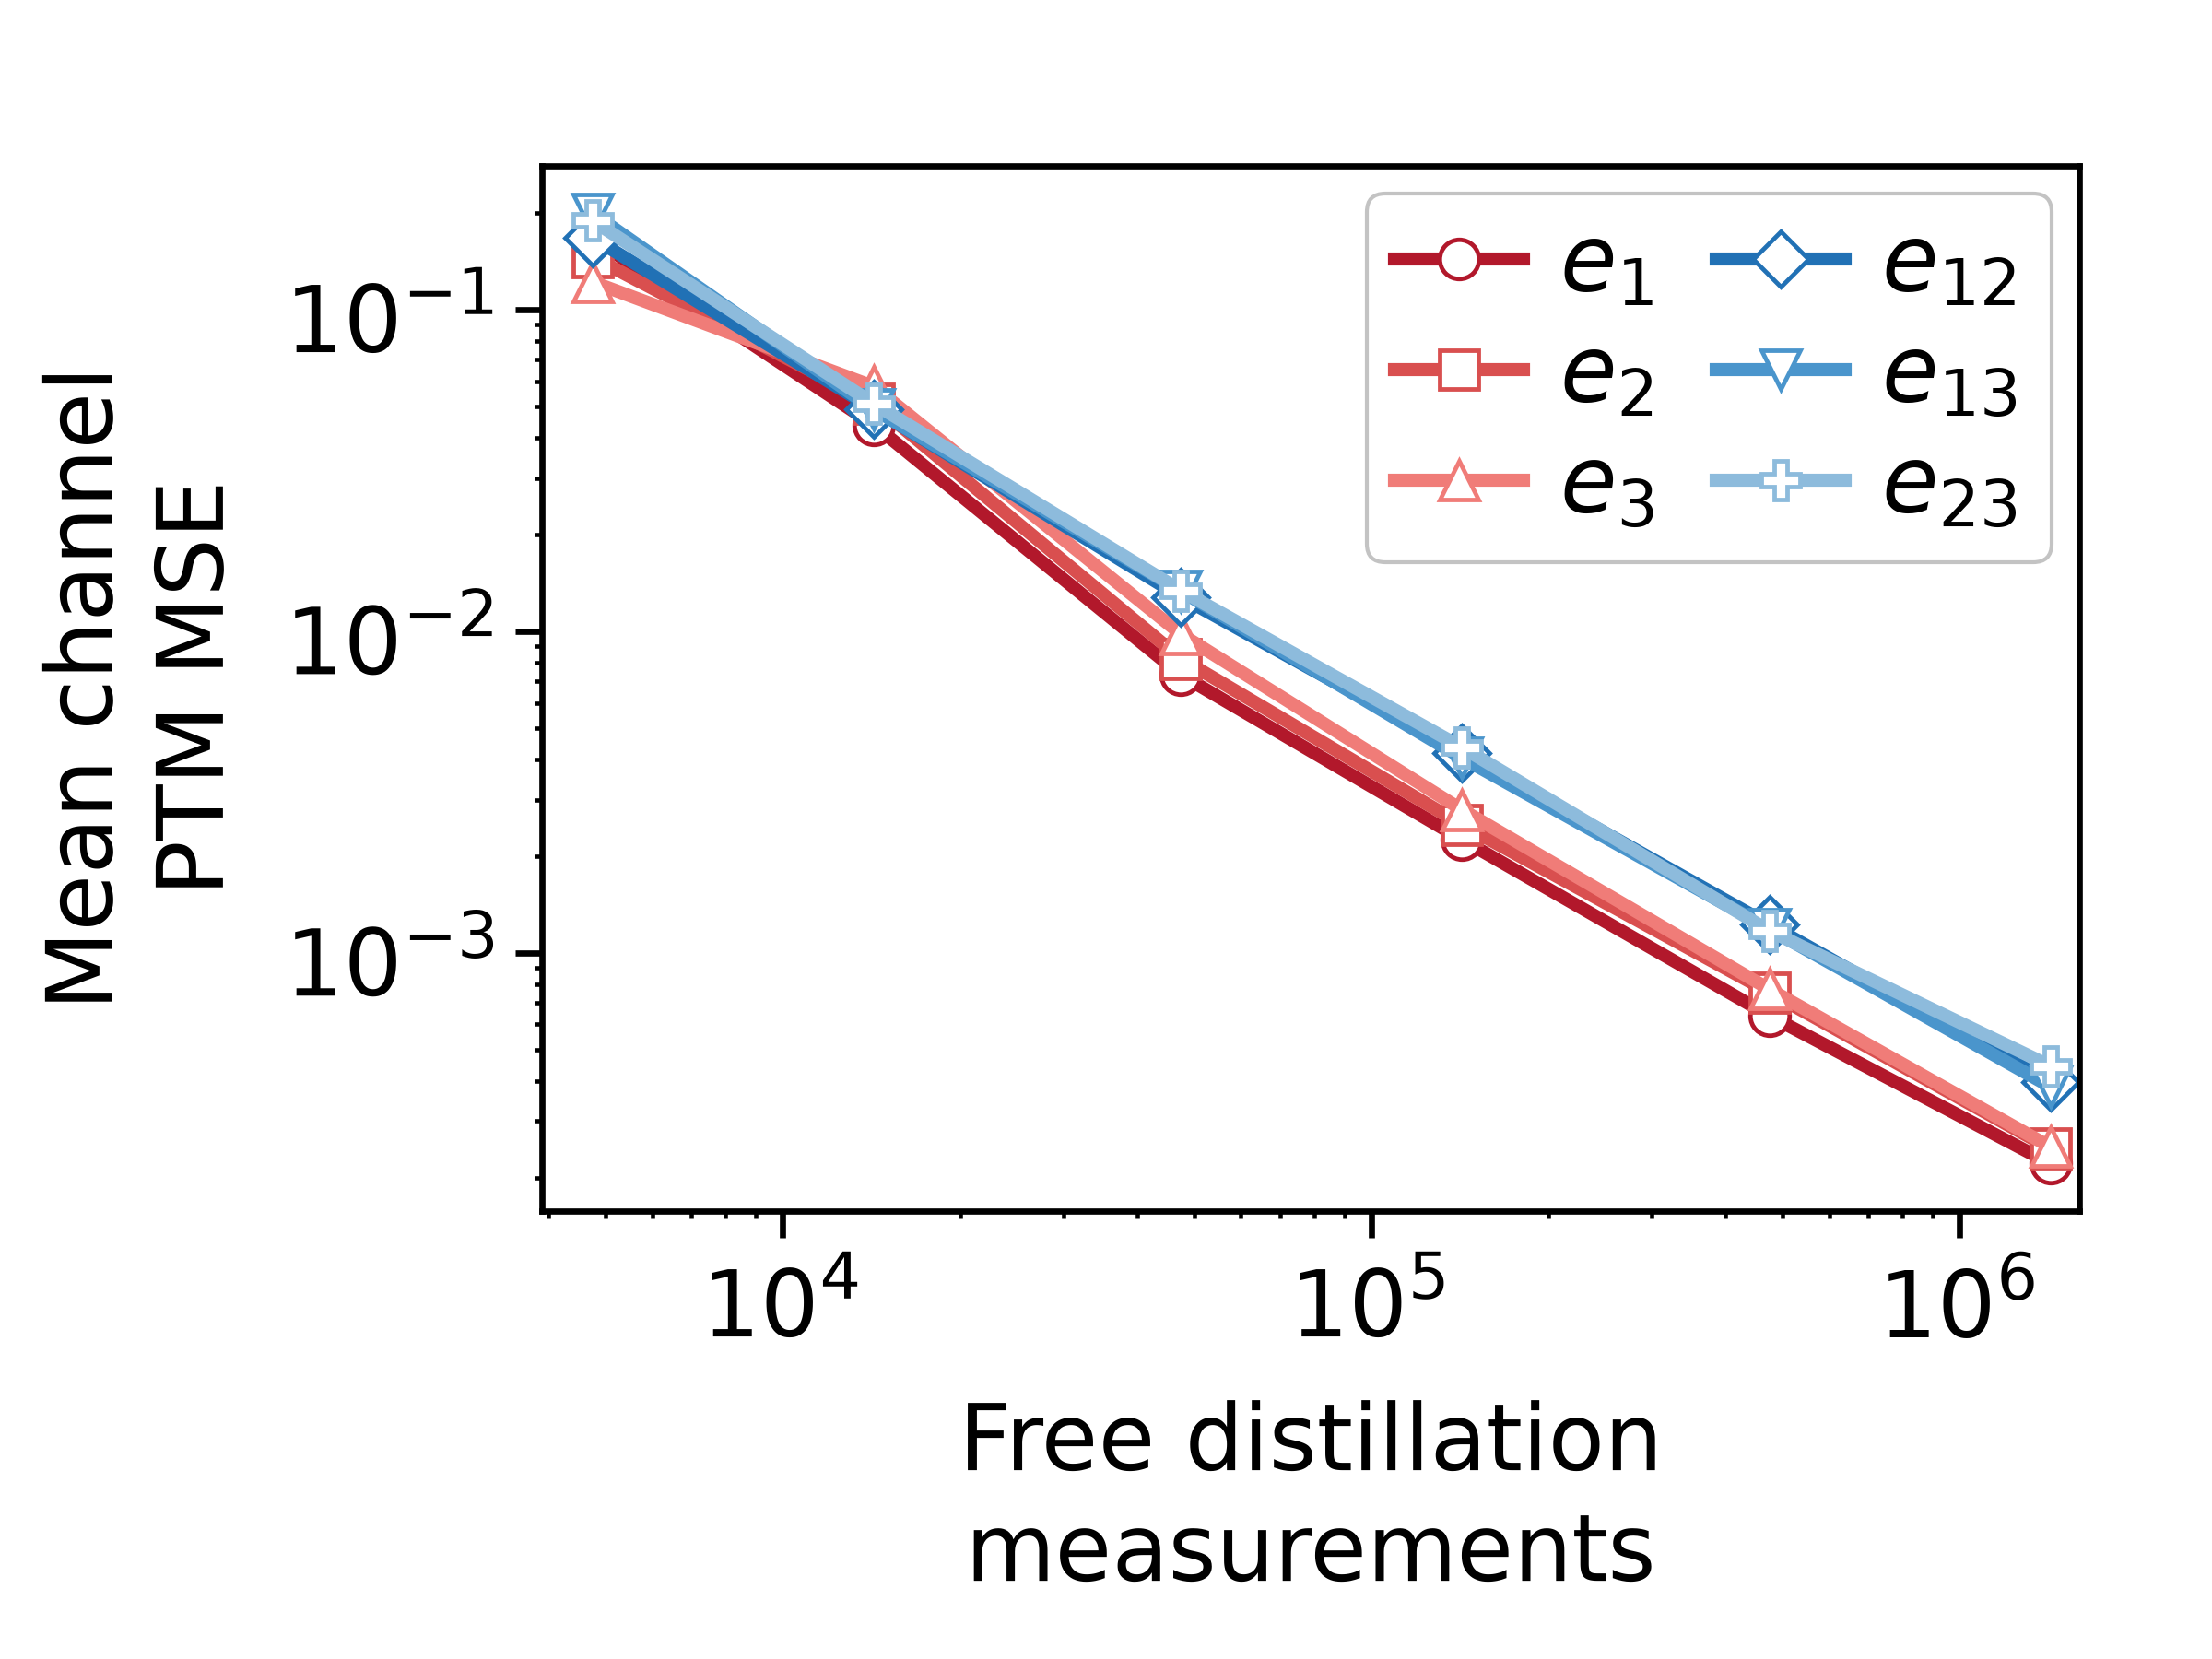
\includegraphics[width=\linewidth]{figures/triangle_sixlink.png}
\caption{Mean per-channel PTM MSE.}
\label{fig:triangle-edge-mse}
\end{subfigure}

\caption{Network topology and tomography performance in a six-link
triangular network.
(a) Peripheral monitors $N_1,N_2,N_3$ connect to internal nodes
$C_1,C_2,C_3$. Colored arrows illustrate an effective star centered
at $C_1$, with channels $\mathcal P_1$,
$\mathcal P_2\circ\mathcal P_{12}$, and
$\mathcal P_3\circ\mathcal P_{13}$.
Analogous constructions at $C_2$ and $C_3$ provide the observations
used for the two-stage reconstruction.
(b) Mean PTM MSE versus the number of distillation measurements
reused for tomography. Red curves represent the outer channels
$e_1,e_2,e_3$, and blue curves represent the inner channels
$e_{12},e_{13},e_{23}$.}
\label{fig:triangle-network-results}
\end{figure}
We apply JCE to three effective stars centered at
$C_1$, $C_2$, and $C_3$.
For example, the star centered at $C_1$ has effective
channels $\mathcal P_1$, $\mathcal P_2\circ\mathcal P_{12}$,
and $\mathcal P_3\circ\mathcal P_{13}$.
For each effective star, we perform two unicast
double-selection configurations and two modified
Mergecast double-selection configurations, with and
without Clifford dressing.
In the first stage, we estimate the outer channels
and the composite branches.
In the second stage, we recover the internal-channel
parameters by dividing the estimated composite-branch
PTM parameters by the corresponding outer-channel
estimates.
Consequently, estimation errors in the outer channels
also propagate into the internal-channel estimates.

Fig.~\ref{fig:triangle-edge-mse} reports the MSE of
each channel, averaged over its three Pauli components
and the algebraically valid repetitions.
The horizontal axis counts the measurements performed
during distillation and reused for tomography,
denoted as \emph{free distillation measurements}.
One complete round across the three effective stars
executes twelve configurations and measures
48 qubits.

The MSE decreases overall for all six channels as the
measurement budget increases.
In this setting, the outer channels exhibit lower
MSE than the internal channels, consistent with
the additional error propagation introduced by
the second reconstruction stage.
These results demonstrate the applicability of
the proposed reconstruction procedure to a network
beyond the three-link star topology.










